%Standardní zobrazovací řetězec a realizace jeho jednotlivých kroků. Gouraudovo a Phongovo stínování. Řešení viditelnosti. Grafický standard OpenGL: stručná charakteristika.
\subsection{Standardní zobrazovací řetěz}
\begin{itemize}
	\item Klade důraz na rychlost nikoli na kvalitu.
	\item Realizuje ho OpenGL.
\end{itemize}
\begin{figure}[H]
\centering
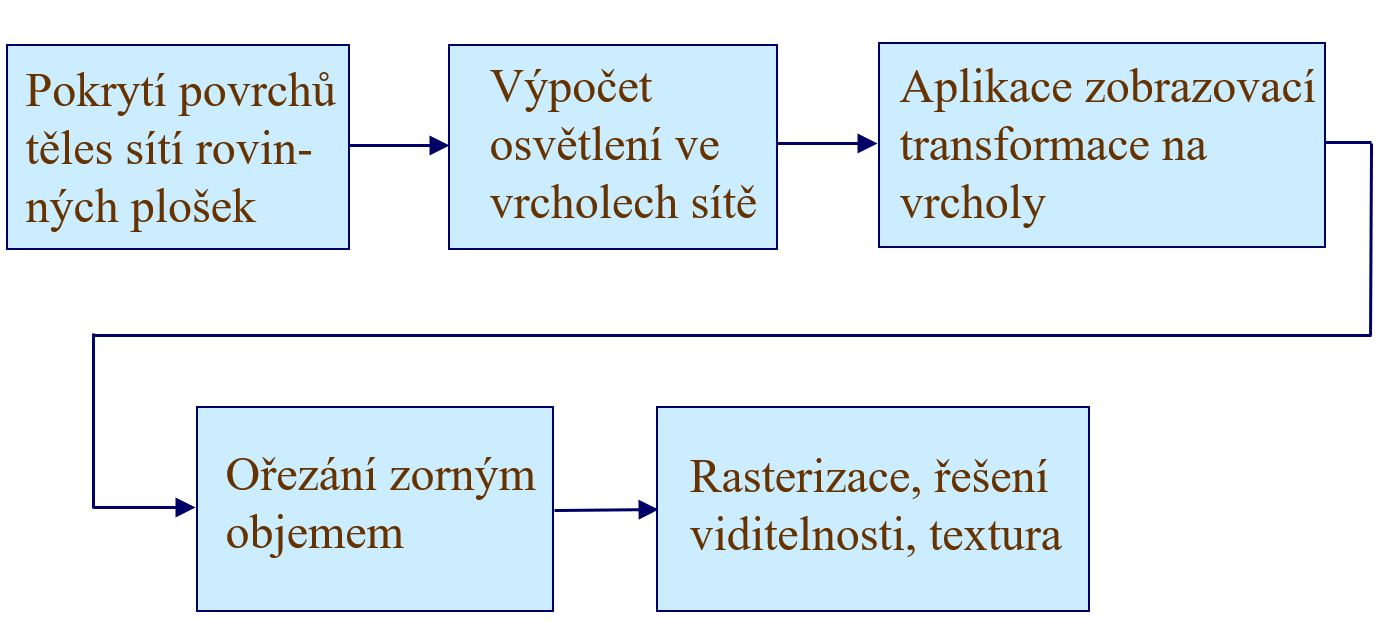
\includegraphics[width=0.8\textwidth]{assets/5_retezec}
\end{figure}

\begin{itemize}
	\item  \textbf{Pokrytí povrchu objektů sítí rovinných plošek:}
	\begin{itemize}
		\item Ploškami bývají nejčastěji trojúhelníky nebo čtyřúhelníky.
		\item Pro objekty ve tvaru mnohostěnu je takové dělní vcelku samozřejmé.
		\item K přesnějšímu výpočtu barev bývá, ale někdy dělení na plošky jemnější.
		\item Někdy síť rovinných plošek žádaný povrch pouze aproximuje.
	\end{itemize}
	\item \textbf{Výpočet osvětlení ve vrcholech sítě}
	\item k tomu známe:
	\begin{itemize}
		\item Polohu, intenzitu a barvu světelných zdrojů.
		\item Souřadnice vrcholů ($P$), normál ($n$) a konstanty popisující optické vlastnosti materiálu ($O_a, O_d, O_s$)
		\begin{figure}[H]
		\centering
		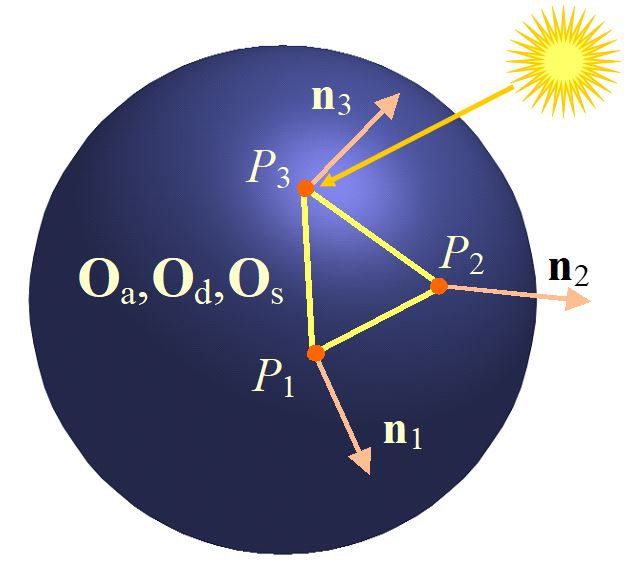
\includegraphics[width=0.5\textwidth]{assets/5_vypocet_barevneho_vjemu}
		\end{figure}
	\end{itemize}
	\item \textbf{Aplikace zobrazovací transformace na vrcholy}
	\begin{itemize}
		\item Oblíbenou technikou je středové promítání. To je zadáno:
		\begin{itemize}
			\item Polohou průmětny.
			\item Polohou středu promítání.
		\end{itemize}
		\begin{figure}[H]
		\centering
		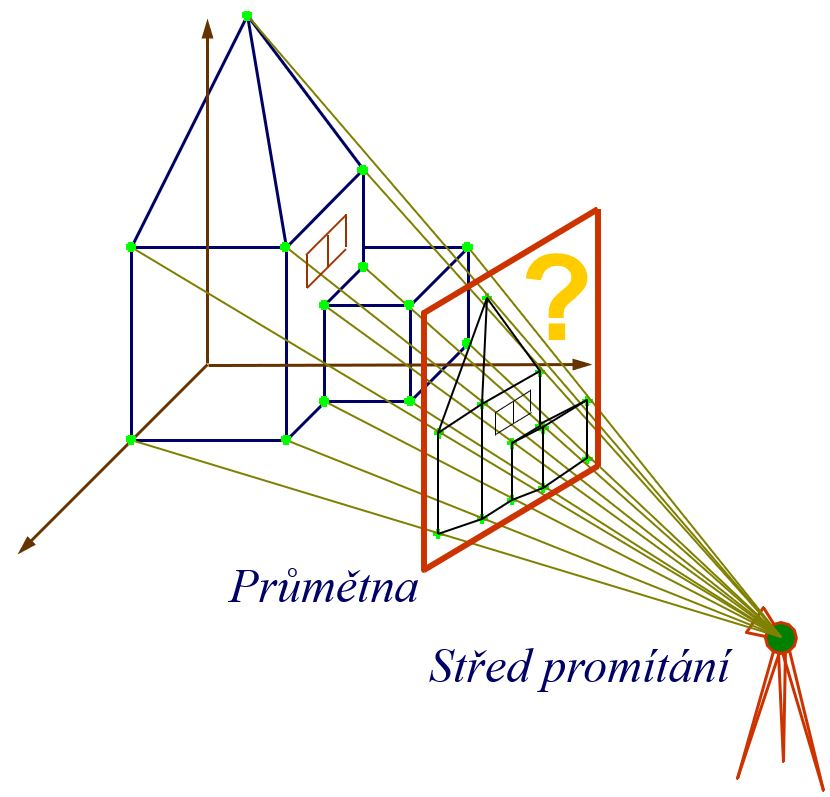
\includegraphics[width=0.5\textwidth]{assets/5_stred_promitani}
		\end{figure}
	\end{itemize}
	\item \textbf{Ořezání zorným objemem}
	\begin{itemize}
		\item Objekty nebo jejich části, nacházející se mimo zorný objem (obvykle jehlan) jsou odstraněny.
	\end{itemize}
		\begin{figure}[H]
		\centering
		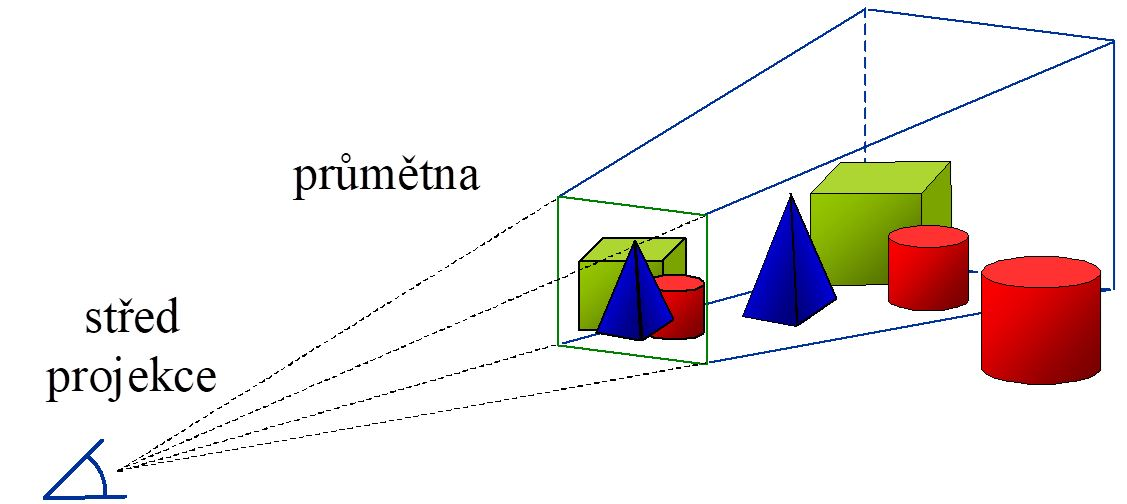
\includegraphics[width=0.5\textwidth]{assets/5_orezani_zornym_pole}
		\end{figure}
	%\begin{itemize}
	\item \textbf{Rasterizace plošek}
	\begin{itemize}
		\item Postupně zpracovávány všechny plošky.
		\item Pro každou plošku rozsvěceny všechny její pixely.
		\item Barva každého pixelu se stanoví interpolací mezi hodnotami ve vrcholech.
		\begin{figure}[H]
		\centering
		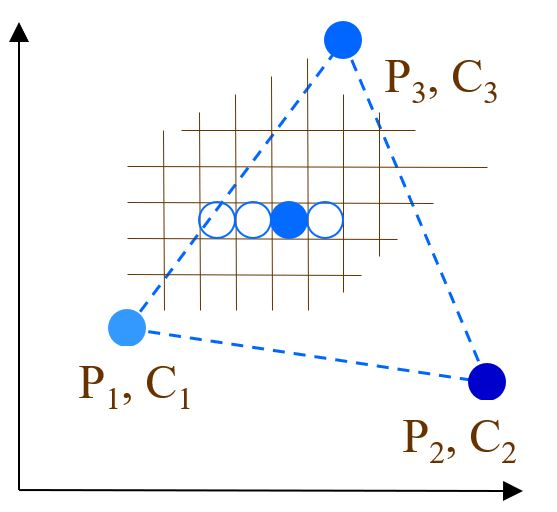
\includegraphics[width=0.5\textwidth]{assets/5_rasterizace_plosek}
		\end{figure}
	\end{itemize}
	\item \textbf{Řešení viditelnosti (z--buffer)}
	\begin{itemize}
		\item Pro rozhodnutí viditelnosti se použijí hodnoty souřadnice $z$ (zde je $z_1 > z_2$).
		\item Před řešením viditelnosti bývá centrálním promítání převedeno na rovnoběžné.
		\begin{figure}[H]
		\centering
		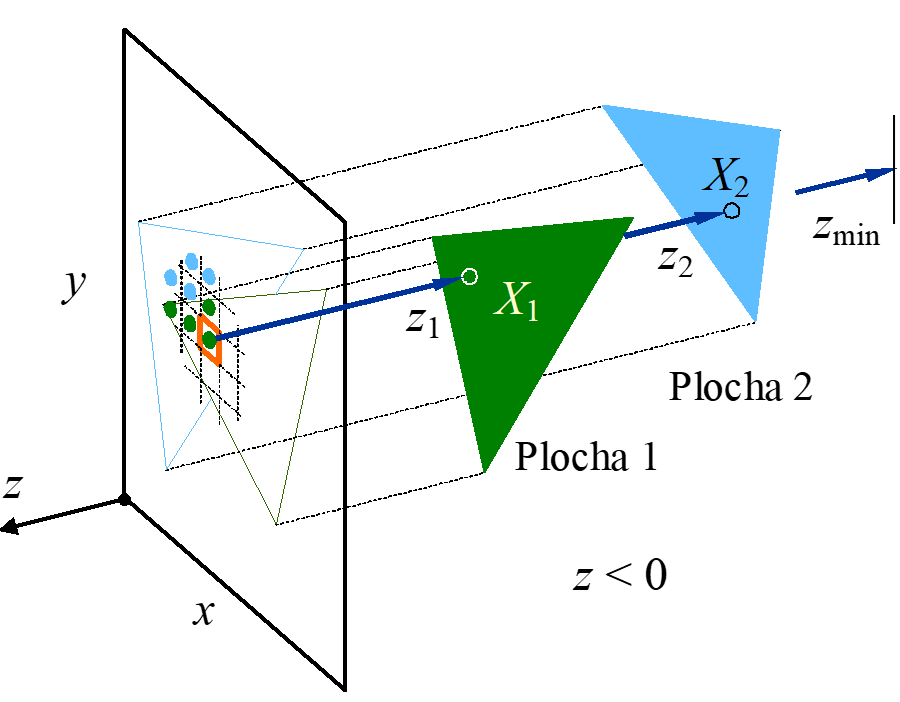
\includegraphics[width=0.5\textwidth]{assets/5_pip_zbuffer}
		\end{figure}
	\end{itemize}
	\item \textbf{Nanášení textury}
	\begin{itemize}
		\item Vzhled obrázků lze vylepšit nánášením textury.
	\end{itemize}
\end{itemize}